\def\year{2022}\relax
%File: formatting-instructions-latex-2022.tex
%release 2022.1
\documentclass[letterpaper]{article} % DO NOT CHANGE THIS
\usepackage{aaai22}  % DO NOT CHANGE THIS
\usepackage{times}  % DO NOT CHANGE THIS
\usepackage{helvet}  % DO NOT CHANGE THIS
\usepackage{courier}  % DO NOT CHANGE THIS
\usepackage{hyperref}
\usepackage[hyphens]{url}  % DO NOT CHANGE THIS
\usepackage{graphicx} % DO NOT CHANGE THIS
\urlstyle{rm} % DO NOT CHANGE THIS
\def\UrlFont{\rm}  % DO NOT CHANGE THIS
\usepackage{natbib}  % DO NOT CHANGE THIS AND DO NOT ADD ANY OPTIONS TO IT
\usepackage{caption} % DO NOT CHANGE THIS AND DO NOT ADD ANY OPTIONS TO IT
\DeclareCaptionStyle{ruled}{labelfont=normalfont,labelsep=colon,strut=off} % DO NOT CHANGE THIS
\frenchspacing  % DO NOT CHANGE THIS
\setlength{\pdfpagewidth}{8.5in}  % DO NOT CHANGE THIS
\setlength{\pdfpageheight}{11in}  % DO NOT CHANGE THIS
%
% These are recommended to typeset algorithms but not required. See the subsubsection on algorithms. Remove them if you don't have algorithms in your paper.
\usepackage{algorithm}
\usepackage{algorithmic}

%
% These are are recommended to typeset listings but not required. See the subsubsection on listing. Remove this block if you don't have listings in your paper.
\usepackage{newfloat}
\usepackage{listings}
\lstset{%
	basicstyle={\footnotesize\ttfamily},% footnotesize acceptable for monospace
	numbers=left,numberstyle=\footnotesize,xleftmargin=2em,% show line numbers, remove this entire line if you don't want the numbers.
	aboveskip=0pt,belowskip=0pt,%
	showstringspaces=false,tabsize=2,breaklines=true}
\floatstyle{ruled}
\newfloat{listing}{tb}{lst}{}
\floatname{listing}{Listing}
%
%\nocopyright
%
% PDF Info Is REQUIRED.
% For /Title, write your title in Mixed Case.
% Don't use accents or commands. Retain the parentheses.
% For /Author, add all authors within the parentheses,
% separated by commas. No accents, special characters
% or commands are allowed.
% Keep the /TemplateVersion tag as is
\pdfinfo{
/Title (Modified ResNet-18)
/Author (AAAI Press Staff, Pater Patel Schneider, Sunil Issar, J. Scott Penberthy, George Ferguson, Hans Guesgen, Francisco Cruz, Marc Pujol-Gonzalez)
/TemplateVersion (2022.1)
}

% DISALLOWED PACKAGES
% \usepackage{authblk} -- This package is specifically forbidden
% \usepackage{balance} -- This package is specifically forbidden
% \usepackage{color (if used in text)
% \usepackage{CJK} -- This package is specifically forbidden
% \usepackage{float} -- This package is specifically forbidden
% \usepackage{flushend} -- This package is specifically forbidden
% \usepackage{fontenc} -- This package is specifically forbidden
% \usepackage{fullpage} -- This package is specifically forbidden
% \usepackage{geometry} -- This package is specifically forbidden
% \usepackage{grffile} -- This package is specifically forbidden
% \usepackage{hyperref} -- This package is specifically forbidden
% \usepackage{navigator} -- This package is specifically forbidden
% (or any other package that embeds links such as navigator or hyperref)
% \indentfirst} -- This package is specifically forbidden
% \layout} -- This package is specifically forbidden
% \multicol} -- This package is specifically forbidden
% \nameref} -- This package is specifically forbidden
% \usepackage{savetrees} -- This package is specifically forbidden
% \usepackage{setspace} -- This package is specifically forbidden
% \usepackage{stfloats} -- This package is specifically forbidden
% \usepackage{tabu} -- This package is specifically forbidden
% \usepackage{titlesec} -- This package is specifically forbidden
% \usepackage{tocbibind} -- This package is specifically forbidden
% \usepackage{ulem} -- This package is specifically forbidden
% \usepackage{wrapfig} -- This package is specifically forbidden
% DISALLOWED COMMANDS
% \nocopyright -- Your paper will not be published if you use this command
% \addtolength -- This command may not be used
% \balance -- This command may not be used
% \baselinestretch -- Your paper will not be published if you use this command
% \clearpage -- No page breaks of any kind may be used for the final version of your paper
% \columnsep -- This command may not be used
% \newpage -- No page breaks of any kind may be used for the final version of your paper
% \pagebreak -- No page breaks of any kind may be used for the final version of your paperr
% \pagestyle -- This command may not be used
% \tiny -- This is not an acceptable font size.
% \vspace{- -- No negative value may be used in proximity of a caption, figure, table, section, subsection, subsubsection, or reference
% \vskip{- -- No negative value may be used to alter spacing above or below a caption, figure, table, section, subsection, subsubsection, or reference

\setcounter{secnumdepth}{0} %May be changed to 1 or 2 if section numbers are desired.

% The file aaai22.sty is the style file for AAAI Press
% proceedings, working notes, and technical reports.
%

% Title

% Your title must be in mixed case, not sentence case.
% That means all verbs (including short verbs like be, is, using,and go),
% nouns, adverbs, adjectives should be capitalized, including both words in hyphenated terms, while
% articles, conjunctions, and prepositions are lower case unless they
% directly follow a colon or long dash
\title{Modified ResNet \\ A comparison between three proposed ResNet model}
\author{
    %Authors
    % All authors must be in the same font size and format.
    Written by Karan Vora, \textsuperscript{\rm 1}
    Parisima Abdali , \textsuperscript{\rm 2}
    Ajay Tibrewal \textsuperscript{\rm 3}
}
\affiliations{ New York University \\ kv5124@nyu.edu, pa2297@nyu.edu, at5632@nyu.edu \\
\href{https://github.com/parisimaa/modifiedResNet.git}
{\underline{github.com/modifiedResNet}}

}

%Example, Single Author, ->> remove \iffalse,\fi and place them surrounding AAAI title to use it
\iffalse
\title{My Publication Title --- Single Author}
\author {
    Author Name
}
\affiliations{
    Affiliation\\
    Affiliation Line 2\\
    name@example.com
}
\fi

\iffalse
%Example, Multiple Authors, ->> remove \iffalse,\fi and place them surrounding AAAI title to use it
\title{My Publication Title --- Multiple Authors}
\author {
    % Authors
    First Author Name,\textsuperscript{\rm 1}
    Second Author Name, \textsuperscript{\rm 2}
    Third Author Name \textsuperscript{\rm 1}
}
\affiliations {
    % Affiliations
    \textsuperscript{\rm 1} Affiliation 1\\
    \textsuperscript{\rm 2} Affiliation 2\\
    firstAuthor@affiliation1.com, secondAuthor@affilation2.com, thirdAuthor@affiliation1.com
}
\fi


% REMOVE THIS: bibentry
% This is only needed to show inline citations in the guidelines document. You should not need it and can safely delete it.
\usepackage{bibentry}
% END REMOVE bibentry

\begin{document}

\maketitle

\begin{abstract}

\end{abstract}
In this project, we introduce three modified versions of the ResNet model with the primary goal of achieving high accuracy while adhering to a constraint of less than 5 million trainable parameters. To achieve this objective, we conducted extensive experiments, leveraging different parameters and techniques, including active learning rate, efficient optimizer, layer augmentation, and dropouts. We meticulously analyzed the results of our experiments, presenting the findings in this paper. The outcomes of our work may have implications for various applications where model size and computational resources are critical factors.


\section{Introduction}
ResNets, or residual neural networks, are a type of deep learning architecture that have been widely used in computer vision tasks such as image classification, object detection, and segmentation.
 They introduce residual connections that allow information to bypass layers and flow directly to the next layer, which has shown to improve the performance of deep networks.
  In this project, we developed and trained a ResNet architecture on the CIFAR 10 dataset \cite{c:25} with the goal of achieving high accuracy while adhering to a constraint of less than 5 million trainable parameters. To understand the effect of parameter scaling, we experimented with three different architectures, ranging from a small ResNet with 78 thousand parameters to a larger architecture with 4.9 million parameters.
 We utilized data visualization techniques to analyze the results of scaling.  Batch normalization was integrated to improve the training of deep networks. Various optimizers were compared, and it was determined that Stochastic Gradient Descent with momentum, including Nesterov acceleration to regulate the momentum, was the most effective approach, as reported by \cite{c:26}. Additionally, we investigated the impact of dropout layers. The final model met the constraint and demonstrated computational efficiency.
 
\section{ResNet Model}
ResNet is a deep convolutional neural network (CNN) architecture proposed by Kaiming He et al. in 2015 \cite{c:24} to address the challenge of training very deep neural networks. It introduces residual blocks with skip connections, allowing gradients to bypass layers and learn residual mappings, making optimization easier. ResNet typically consists of convolutional, batch normalization, activation, and pooling layers, followed by global average pooling and fully connected output layers. It has multiple variants with increasing depth and capacity, such as ResNet-18, ResNet-34, ResNet-50, ResNet-101, and ResNet-152. ResNet has achieved state-of-the-art performance in various computer vision tasks and is widely used in deep learning applications.

\begin{figure}[htbp]
\captionsetup[subfigure]{justification=centering}
  \centering
  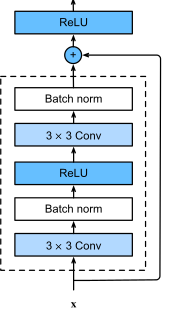
\includegraphics[scale = 0.5]{image/resnet-block.png}
  \caption{ResNet Block}
%  \label{fig:fig2}
\end{figure}

\section{Network Architecture}
The three models, ResNetSmall, ResNetMedium, and ResNetLarge, are variations of the ResNet architecture. The main differences between these three models are the number of layers, the number of filters (or channels) in each layer, and the size of the final fully connected layer.
\subsection{Small Network Layer Summary and Total Parameters}
This model has 3 layers (referred to as "layer1", "layer2", and "layer3") and a final fully connected layer with 64 units (or neurons). The number of filters in the convolutional layers gradually increases from 16 to 64 as we go deeper into the network.

\begin{quote}
\begin{scriptsize}\begin{verbatim}
--------------------------------------------------------
        Layer (type)          Output Shape    Param #
========================================================
            Conv2d-1      [-1, 16, 32, 32]        432
       BatchNorm2d-2      [-1, 16, 32, 32]         32
            Conv2d-3      [-1, 16, 32, 32]      2,304
       BatchNorm2d-4      [-1, 16, 32, 32]         32
            Conv2d-5      [-1, 16, 32, 32]      2,304
       BatchNorm2d-6      [-1, 16, 32, 32]         32
        BasicBlock-7      [-1, 16, 32, 32]          0
            Conv2d-8      [-1, 32, 16, 16]      4,608
       BatchNorm2d-9      [-1, 32, 16, 16]         64
           Conv2d-10      [-1, 32, 16, 16]      9,216
      BatchNorm2d-11      [-1, 32, 16, 16]         64
           Conv2d-12      [-1, 32, 16, 16]        512
      BatchNorm2d-13      [-1, 32, 16, 16]         64
       BasicBlock-14      [-1, 32, 16, 16]          0
           Conv2d-15        [-1, 64, 8, 8]     18,432
      BatchNorm2d-16        [-1, 64, 8, 8]        128
           Conv2d-17        [-1, 64, 8, 8]     36,864
      BatchNorm2d-18        [-1, 64, 8, 8]        128
           Conv2d-19        [-1, 64, 8, 8]      2,048
      BatchNorm2d-20        [-1, 64, 8, 8]        128
       BasicBlock-21        [-1, 64, 8, 8]          0
AdaptiveAvgPool2d-22        [-1, 64, 1, 1]          0
           Linear-23              [-1, 10]        650
=======================================================
Total params: 78,042
Trainable params: 78,042
Non-trainable params: 0
-------------------------------------------------------
Input size (MB): 0.01
Forward/backward pass size (MB): 1.53
Params size (MB): 0.30
Estimated Total Size (MB): 1.84
-------------------------------------------------------
\end{verbatim}\end{scriptsize}
\end{quote}

\begin{figure}[htbp]
\captionsetup[subfigure]{justification=centering}
  \centering
  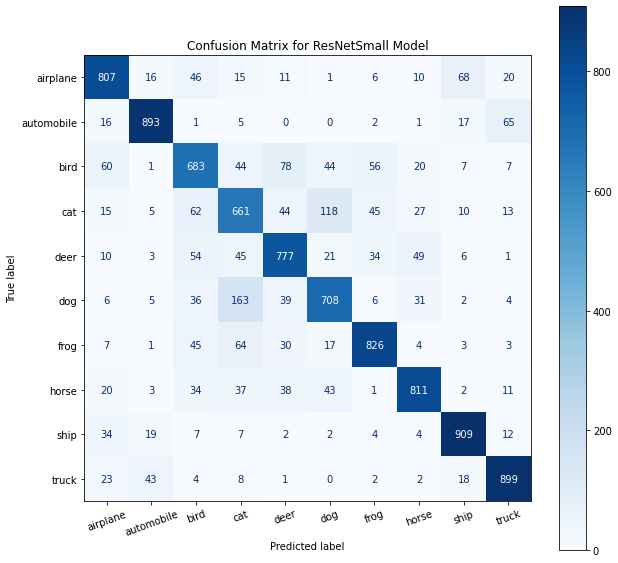
\includegraphics[scale = 0.4]{image/con_small.png}
  \caption{Confusion Matrix SmallModel}
%  \label{fig:fig2}
\end{figure}

\subsection{Medium Network Layer Summary and Total Parameters}
This model has 4 layers (referred to as "layer1", "layer2", "layer3", and "layer4") and a final fully connected layer with 256 units. The number of filters in the convolutional layers gradually increases from 32 to 512 as we go deeper into the network.
\begin{quote}
\begin{scriptsize}\begin{verbatim}
--------------------------------------------------------
        Layer (type)           Output Shape    Param #
========================================================
            Conv2d-1       [-1, 32, 32, 32]       864
       BatchNorm2d-2       [-1, 32, 32, 32]        64
            Conv2d-3       [-1, 32, 32, 32]     9,216
       BatchNorm2d-4       [-1, 32, 32, 32]        64
            Conv2d-5       [-1, 32, 32, 32]     9,216
       BatchNorm2d-6       [-1, 32, 32, 32]        64
        BasicBlock-7       [-1, 32, 32, 32]         0
            Conv2d-8       [-1, 64, 16, 16]    18,432
       BatchNorm2d-9       [-1, 64, 16, 16]       128
           Conv2d-10       [-1, 64, 16, 16]    36,864
      BatchNorm2d-11       [-1, 64, 16, 16]       128
           Conv2d-12       [-1, 64, 16, 16]     2,048
      BatchNorm2d-13       [-1, 64, 16, 16]       128
       BasicBlock-14       [-1, 64, 16, 16]         0
           Conv2d-15        [-1, 128, 8, 8]    73,728
      BatchNorm2d-16        [-1, 128, 8, 8]       256
           Conv2d-17        [-1, 128, 8, 8]   147,456
      BatchNorm2d-18        [-1, 128, 8, 8]       256
           Conv2d-19        [-1, 128, 8, 8]     8,192
      BatchNorm2d-20        [-1, 128, 8, 8]       256
       BasicBlock-21        [-1, 128, 8, 8]         0
           Conv2d-22        [-1, 256, 4, 4]   294,912
      BatchNorm2d-23        [-1, 256, 4, 4]       512
           Conv2d-24        [-1, 256, 4, 4]   589,824
      BatchNorm2d-25        [-1, 256, 4, 4]       512
           Conv2d-26        [-1, 256, 4, 4]    32,768
      BatchNorm2d-27        [-1, 256, 4, 4]       512
       BasicBlock-28        [-1, 256, 4, 4]         0
AdaptiveAvgPool2d-29        [-1, 256, 1, 1]         0
           Linear-30               [-1, 10]     2,570
=======================================================
Total params: 1,228,970
Trainable params: 1,228,970
Non-trainable params: 0
-------------------------------------------------------
Input size (MB): 0.01
Forward/backward pass size (MB): 3.28
Params size (MB): 4.69
Estimated Total Size (MB): 7.98
-------------------------------------------------------

\end{verbatim}\end{scriptsize}
\end{quote}
\begin{figure}[htbp]
\captionsetup[subfigure]{justification=centering}
  \centering
  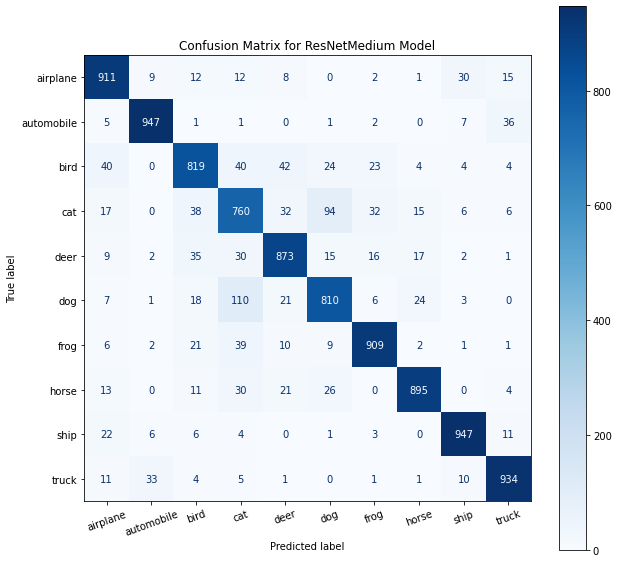
\includegraphics[scale = 0.4]{image/con_medi.png}
  \caption{Confusion Matrix Medium Model}
%  \label{fig:fig2}
\end{figure}
\subsection{Large Network Layer Summary and Total Parameters}
This model has 4 layers (referred to as "layer1", "layer2", "layer3", and "layer4") and a final fully connected layer with 512 units. The number of filters in the convolutional layers gradually increases from 64 to 512 as we go deeper into the network.
\begin{quote}
\begin{scriptsize}\begin{verbatim}
--------------------------------------------------------
        Layer (type)           Output Shape    Param #
========================================================
            Conv2d-1       [-1, 64, 32, 32]      1,728
       BatchNorm2d-2       [-1, 64, 32, 32]        128
            Conv2d-3       [-1, 64, 32, 32]     36,864
       BatchNorm2d-4       [-1, 64, 32, 32]        128
            Conv2d-5       [-1, 64, 32, 32]     36,864
       BatchNorm2d-6       [-1, 64, 32, 32]        128
        BasicBlock-7       [-1, 64, 32, 32]          0
            Conv2d-8      [-1, 128, 16, 16]     73,728
       BatchNorm2d-9      [-1, 128, 16, 16]        256
           Conv2d-10      [-1, 128, 16, 16]    147,456
      BatchNorm2d-11      [-1, 128, 16, 16]        256
           Conv2d-12      [-1, 128, 16, 16]      8,192
      BatchNorm2d-13      [-1, 128, 16, 16]        256
       BasicBlock-14      [-1, 128, 16, 16]          0
           Conv2d-15        [-1, 256, 8, 8]    294,912
      BatchNorm2d-16        [-1, 256, 8, 8]        512
           Conv2d-17        [-1, 256, 8, 8]    589,824
      BatchNorm2d-18        [-1, 256, 8, 8]        512
           Conv2d-19        [-1, 256, 8, 8]     32,768
      BatchNorm2d-20        [-1, 256, 8, 8]        512
       BasicBlock-21        [-1, 256, 8, 8]          0
           Conv2d-22        [-1, 512, 4, 4]  1,179,648
      BatchNorm2d-23        [-1, 512, 4, 4]      1,024
           Conv2d-24        [-1, 512, 4, 4]  2,359,296
      BatchNorm2d-25        [-1, 512, 4, 4]      1,024
           Conv2d-26        [-1, 512, 4, 4]    131,072
      BatchNorm2d-27        [-1, 512, 4, 4]      1,024
       BasicBlock-28        [-1, 512, 4, 4]          0
AdaptiveAvgPool2d-29        [-1, 512, 1, 1]          0
           Linear-30               [-1, 10]      5,130
========================================================
Total params: 4,903,242
Trainable params: 4,903,242
Non-trainable params: 0
--------------------------------------------------------
Input size (MB): 0.01
Forward/backward pass size (MB): 6.57
Params size (MB): 18.70
Estimated Total Size (MB): 25.28
--------------------------------------------------------
\end{verbatim}\end{scriptsize}
\end{quote}\textbf{}
\begin{figure}[htbp]
\captionsetup[subfigure]{justification=centering}
  \centering
  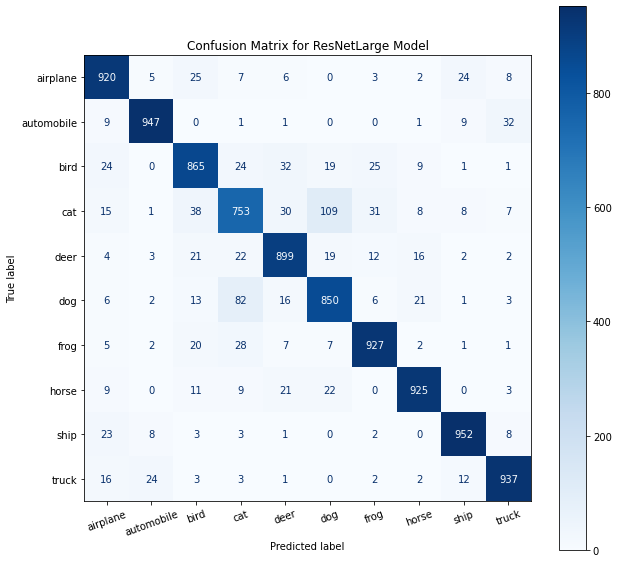
\includegraphics[scale = 0.4]{image/con_large.png}
  \caption{Confusion Matrix LargeModel}
%  \label{fig:fig2}
\end{figure}

\subsubsection{Basic block}
The BasicBlock class in PyTorch is a building block for the ResNet neural network architecture. It consists of two convolutional layers, batch normalization, and ReLU activation. The first convolutional layer applies a 3x3 convolution and batch normalization, followed by a second convolutional layer with shortcut connections. The output is passed through ReLU activation and returned as the output of the BasicBlock layer.
\subsubsection{Skip Connection in basic block}
The skip connection in the BasicBlock is implemented through a shortcut layer as we can see in Figure 1, which directly connects the input to the output of the block through element-wise addition. This helps the network learn identity mappings, which can improve gradient propagation in deep networks. The shortcut connection is only applied when input and output have different dimensions, and it consists of Conv2d and BatchNorm2d layers to adjust dimensions and channels. If input and output have the same dimensions, the shortcut layer is an identity mapping with no additional computation.
\subsubsection{Optimizer}
After experimenting with various optimizers for training our model, we concluded that using Stochastic Gradient Descent (SGD) with Momentum and Nesterov Accelerated Gradient (NAG) resulted in the highest accuracy. The optimizer configuration with the highest accuracy with $learning rate = 0.01, momentum = 0.9 $ achieved an accuracy of above 94\% on the large model. Other optimizers such as Adam achieved an accuracy of about 85\%.
\subsubsection{Hyper-parameters}
In the project, we utilized several hyperparameters to configure the learning rate (LR) during the training process. The LR was set to a minimum value of 1e-6 and a maximum value of 1e-2, spanning a wide range to enable effective model optimization. We trained the model for a total of 30 epochs, which represents the number of complete passes through the entire training dataset. To dynamically adjust the LR during training, we employed a cyclic learning rate (CLR) strategy. The CLR was implemented using the CyclicLR scheduler from the PyTorch optimizer module.

\subsubsection{Criterion}
In our project, we used the cross-entropy loss (denoted as nn.CrossEntropyLoss() in PyTorch) as the objective function, or criterion, for training our model. The cross-entropy loss is a common choice for multi-class classification tasks, such as image classification, where the goal is to classify input data into multiple mutually exclusive classes. It measures the dissimilarity between the predicted class probabilities and the true class labels and provides a scalar value that reflects the model's performance. During training, the model's parameters are updated based on the gradient of the cross-entropy loss, with the aim of minimizing the loss and improving the model's accuracy in predicting the correct class labels.

\subsubsection{Data Augmentation}
In our project, we used data augmentation techniques to enhance the training dataset and improve the model's ability to generalize to unseen data. We used the torchvision.transforms module in PyTorch to apply various image transformations to the input images before feeding them into the model for training.\\
For the training dataset, we applied the following transformations using the transforms.Compose() function: \\
Randomly rotating the image by a maximum of 5 degrees in a counter-clockwise or clockwise direction, which introduces diversity in the orientation of the images in the training set. \\
Horizontally flipping the image with a probability of 0.5, introduces diversity in the horizontal orientation of the images in the training set. \\
Randomly cropping a 32x32 pixel patch from the image with a padding of 2 pixels, introduces diversity in the spatial location of the images in the training set. \\

\section{Evaluation}
The three proposed models were evaluated using multiple metrics. Cross Entropy Loss was chosen for training purposes, and the models were compared based on their training loss and accuracy across epochs. As shown in Figure 5 and Figure 6, the large model outperformed the small model, exhibiting the lowest loss and highest accuracy throughout the epochs. To further visualize the results, confusion matrices were plotted in Figures 2, 3, and 4. It was observed that certain labels, such as 'airplane' and 'automobile', were classified more accurately by all three models, while the 'cat' label had the highest misclassification rate, often being misclassified as 'dog'. Overall, the larger model demonstrated better performance in terms of both accuracy and loss, with the other models showing similar performance in comparison.
\begin{figure}[htbp]
\captionsetup[subfigure]{justification=centering}
  \centering
  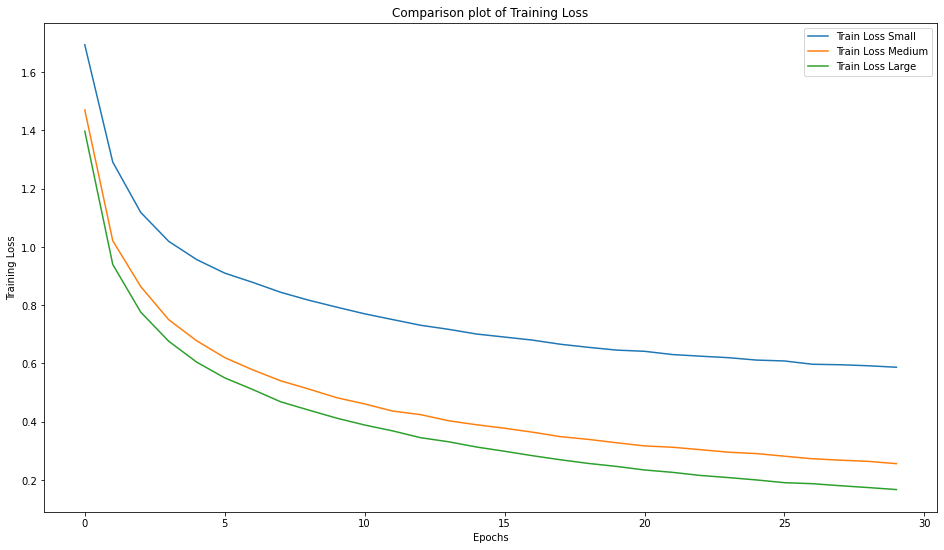
\includegraphics[scale = 0.25]{image/train.png}
  \caption{Training loss comparison of the three models}
%  \label{fig:fig5}
\end{figure}

\begin{figure}[htbp]
\captionsetup[subfigure]{justification=centering}
  \centering
  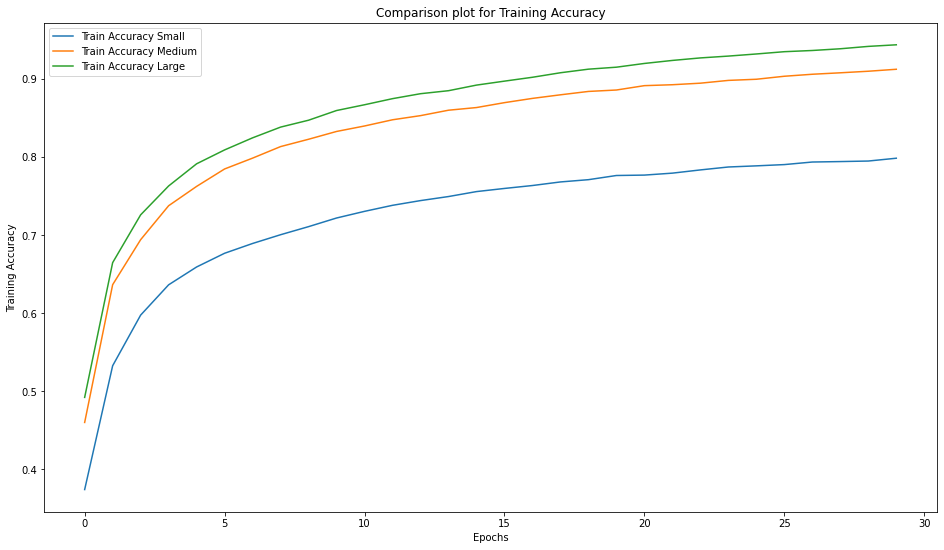
\includegraphics[scale = 0.25]{image/train_acc.png}
  \caption{Training accuracy comparison of the three models}
%  \label{fig:fig6}
\end{figure}

\begin{figure}[htbp]
\captionsetup[subfigure]{justification=centering}
  \centering
  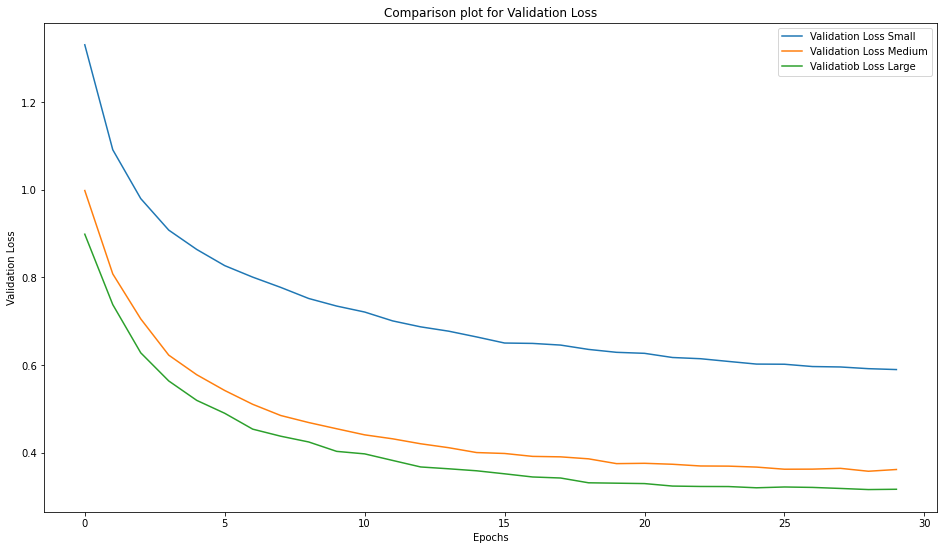
\includegraphics[scale = 0.25]{image/val_loss.png}
  \caption{Test loss comparison of the three models}
%  \label{fig:fig7}
\end{figure}

\begin{figure}[htbp]
\captionsetup[subfigure]{justification=centering}
  \centering
  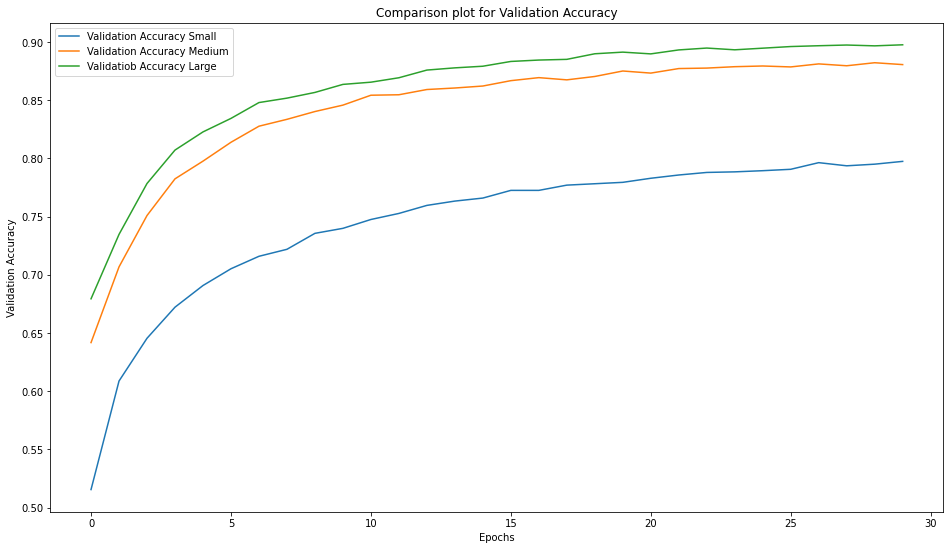
\includegraphics[scale = 0.25]{image/val_acc.png}
  \caption{Test accuracy comparison of the three models}
%  \label{fig:fig8}
\end{figure}

\begin{table}[h]
    \centering
    \caption{Train and test accuracy comparisons for models}
    \label{tab:example}
    \resizebox{0.95\columnwidth}{!}{
    \begin{tabular}{|c|c|c|c|}
        \hline
        Models &Parameters & Train Accuracy & Test Accuracy \\
        \hline
        ResNetSmall & $78,042$ & $79.18\%$ & $79.40\%$\\
        \hline 
        ResNetMedium & $1,228,970$ & $91.06\%$ & $87.99\%$\\
        \hline
        ResNetLarge & $4,903,242$ & $94.16\%$ & $89.66\%$ \\
        \hline
    \end{tabular}
    }
\end{table}

\section{System Specification}
NYU HPC VM \\
CPU: 8 Virtualized Cores of Intel Xeon-Platinum 8286 \\
GPU: Nvidia Quadro RTX 8000 \\
System Memory: 96 GB \\
Python Version: 3.8.6 \\
CUDA version: v11.8 \\
Torch Version: 2.0.0 \\

\section{Acknowledgment}
We would like to acknowledge the use of OpenAI's GPT-3.5 language model, commonly referred to as ChatGPT, for providing assistance with generating content for certain sections of this report.

\bibliography{aaai22}. \\
% \bibentry{c:25}.
%\nobibliography{aaai22}

\end{document}
